\chapter{Chemical Species, Natural and Synthetic}\label{ch:g10:chemical-species}

A spoonful of vanilla ice cream. Its flavour may come from the black pods
of a tropical orchid, picked, cured and soaked in alcohol for months; or
it may come from a factory that makes the flavour from wood pulp or from
oil. Taste the two side by side and the main flavour is the same --- for
a good reason: the \omterm{def:g7:atoms-and-molecules:molecule}{molecule} that tastes of vanilla, vanillin, is exactly
the same \omterm{def:g7:atoms-and-molecules:molecule}{molecule}, whichever way it was obtained. This chapter shows how
chemists take a species out of a plant, how they make it, and how they
check that what they have is what they think.

\begin{recall}
A \omterm{def:g6:pure-substances-and-mixtures:species}{chemical species} is one particular kind of substance; a \omterm{def:g6:pure-substances-and-mixtures:pure-substance}{pure substance}
holds one species and has fixed constants, such as its melting and
boiling temperatures (\cref{ch:g6:pure-substances-and-mixtures}). Liquids
are \omterm{def:g6:solutions-and-solubility:miscible}{miscible} or \omterm{def:g6:solutions-and-solubility:miscible}{immiscible}, and each \omterm{def:g6:solutions-and-solubility:solute}{solute} has its own \omterm{def:g6:solutions-and-solubility:solubility}{solubility} in
each \omterm{def:g6:solutions-and-solubility:solute}{solvent} (\cref{ch:g6:solutions-and-solubility}). \omterm{def:g7:identifying-substances:chromatography}{Paper
chromatography} separates the dyes of a \omterm{def:g6:pure-substances-and-mixtures:mixture}{mixture}
(\cref{ch:g7:identifying-substances}).
\end{recall}

\begin{omfigure}
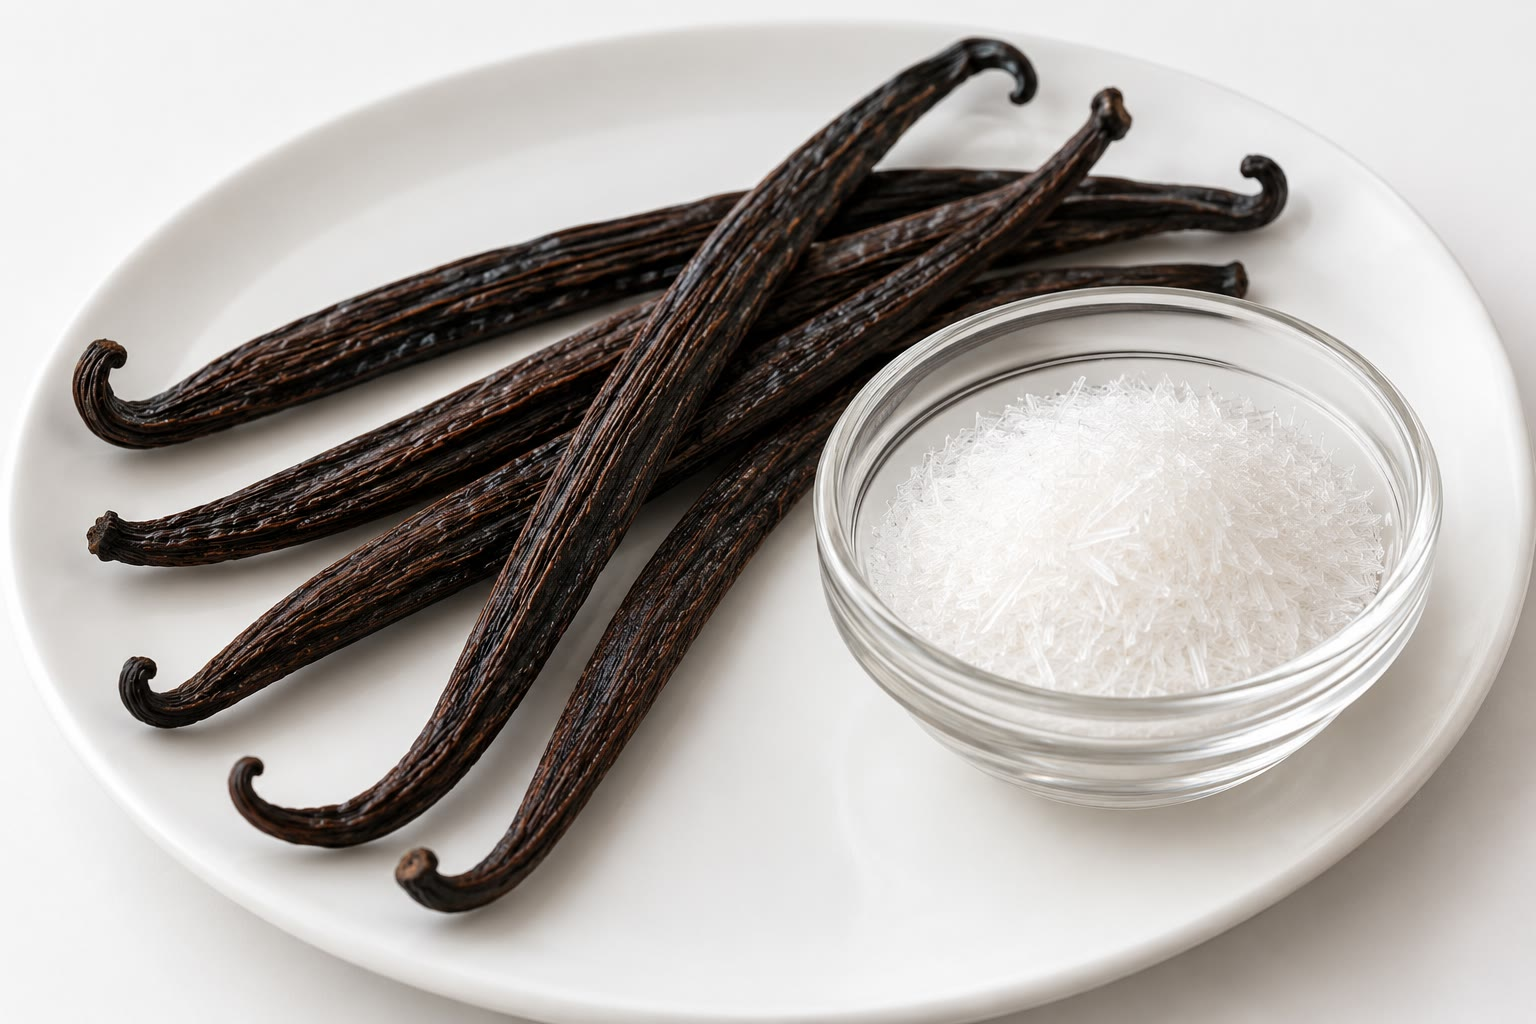
\includegraphics[width=0.55\linewidth]{images/book1/ai/g10-vanilla.jpg}

{\small Vanilla pods and white crystals of vanillin: the same \omterm{def:g7:atoms-and-molecules:molecule}{molecule},
from a plant or from a factory.}
\end{omfigure}

\section{Natural and synthetic species}

\begin{definition}[Natural and synthetic species]\label{def:g10:chemical-species:natural}
A \emph{natural species}\index{natural species} is a \omterm{def:g6:pure-substances-and-mixtures:species}{chemical species}
made by a living being or found as such in nature. A \emph{synthetic
species}\index{synthetic species} is made by chemists from other species
by \omterm{def:g7:chemical-reactions:reaction}{chemical reactions}. A synthetic species may be identical to a natural
one (synthetic vanillin), or have no counterpart in nature (most
medicines and \omterm{def:g8:plastics:plastic}{plastics}).
\end{definition}

\begin{proposition}[Same species, same properties]\label{prop:g10:chemical-species:same}
A \omterm{def:g6:pure-substances-and-mixtures:species}{chemical species} has the same properties whatever its origin:
vanillin made in a factory and vanillin extracted from a pod have the same
formula, the same melting point, the same smell. What can differ is what
comes with it: a natural extract is a \omterm{def:g6:pure-substances-and-mixtures:mixture}{mixture}, with many other species
that change its taste.
\end{proposition}

\begin{history}[From willow bark to aspirin, 1828--1899]
For centuries, willow bark was chewed against fever and pain. In 1828 a
chemist extracted from it the active species, salicin; chemists then
turned it into salicylic acid, which works but irritates the stomach. In
1897, at a dye and drug company, Felix Hoffmann made a gentler \omterm{def:g10:chemical-species:natural}{synthetic
species} from salicylic acid: acetylsalicylic acid, sold from 1899 as
aspirin. Aspirin has no natural source: it is a purely \omterm{def:g10:chemical-species:natural}{synthetic species}.
\end{history}

\section{Extracting a species}

\begin{definition}[Extraction and liquid--liquid extraction]\label{def:g10:chemical-species:extraction}
An \emph{extraction}\index{extraction} takes a \omterm{def:g6:pure-substances-and-mixtures:species}{chemical species} out of
the material that contains it, usually by dissolving it in a well-chosen
\omterm{def:g6:solutions-and-solubility:solute}{solvent}. In a \emph{liquid--liquid extraction}\index{liquid--liquid
extraction}, a species dissolved in one liquid is transferred into a
second liquid, \omterm{def:g6:solutions-and-solubility:miscible}{immiscible} with the first, in which it \omterm{def:g2:mixing-and-dissolving:dissolve}{dissolves} better;
the two liquids are then separated in a separating funnel.
\end{definition}

\begin{example}[Everyday extractions]\label{ex:g10:chemical-species:everyday}
Making tea is an \omterm{def:g10:chemical-species:extraction}{extraction} with hot water (infusion); soaking vanilla
pods in alcohol is an \omterm{def:g10:chemical-species:extraction}{extraction} with ethanol (maceration); boiling
vegetables to make a stock is another (decoction).
\end{example}


\begin{definition}[Distillation and hydrodistillation]\label{def:g10:chemical-species:distillation}
A \emph{distillation}\index{distillation} heats a liquid \omterm{def:g6:pure-substances-and-mixtures:mixture}{mixture} to
boiling, turns the vapour back into liquid in a condenser cooled by
running water, and collects this liquid, the distillate. A
\emph{hydrodistillation}\index{hydrodistillation} boils a plant material
in water: the steam carries away the fragrant species of the plant,
which separate from the water in the distillate as an oily layer, the
essential oil.
\end{definition}

\begin{omfigure}
\begin{tikzpicture}[font=\small, scale=0.95]
  \pic[transform shape] at (0,0) {heatingmantle};
  \pic[transform shape] at (0,0) {rbflask={0.55}{omWater!70}};
  \foreach \x/\y in {-0.45/0.35,-0.1/0.55,0.3/0.3,0.5/0.7,-0.6/0.75,0.1/0.9,-0.25/0.2}
    \fill[green!45!black!70] (\x,\y) ellipse (0.09 and 0.04);
  \pic[transform shape] (s) at (0,3.0) {stillhead};
  \pic[transform shape] at ($(s-top)+(0,-0.75)$) {thermometer};
  \pic[transform shape, rotate=-20] (c) at (s-arm) {liebig={3.2}};
  \coordinate (cend) at ($(s-arm)+(-20:3.2)$);
  \pic[transform shape] (a) at (cend) {adapter};
  \pic[transform shape] at ($(a-tip)+(0,-2.3)$) {erlenmeyer={0.18}{omWater!70}};
  \fill[yellow!60!orange!60] ($(a-tip)+(-0.827,-2.3+0.47)$) -- ($(a-tip)+(0.827,-2.3+0.47)$) -- ($(a-tip)+(0.779,-2.3+0.6)$) -- ($(a-tip)+(-0.779,-2.3+0.6)$) -- cycle;
  \draw[<-, omProp, thick] (-0.55,0.55) -- (-2.2,0.9) node[left, text=black, align=right]
    {water and\\ lavender flowers};
  \draw[<-, omProp, thick] (1.35,-0.6) -- (2.2,-1.1) node[right, text=black]
    {heating mantle};
  \draw[<-, omProp, thick] (0.1,4.2) -- (-1.2,4.6) node[left, text=black] {thermometer};
  \draw[<-, omProp, thick] ($(s-arm)+(-20:1.6)+(0,0.32)$) -- ++(0.6,1.0) node[above, text=black]
    {condenser, cooled by running water};
  \draw[<-, omProp, thick] ($(a-tip)+(0.4,-1.88)$) -- ++(1.1,0.2) node[right, text=black, align=left]
    {distillate: essential oil\\ floating on water};
\end{tikzpicture}

{\small \omterm{def:g10:chemical-species:distillation}{Hydrodistillation} of lavender. The steam carries the essential oil
into the condenser; the distillate separates into a thin layer of oil on
top of water.}
\end{omfigure}

\begin{method}[Choosing an extraction solvent]\label{met:g10:chemical-species:solvent}
For a \omterm{def:g10:chemical-species:extraction}{liquid--liquid extraction} of a species from water, the \omterm{def:g6:solutions-and-solubility:solute}{solvent}
must:
\begin{enumerate}
  \item \omterm{def:g2:mixing-and-dissolving:dissolve}{dissolve} the species much better than water does;
  \item be \omterm{def:g6:solutions-and-solubility:miscible}{immiscible} with water, so that two layers form;
  \item be as little hazardous as possible, and easy to remove afterwards
        (a low boiling temperature lets it evaporate).
\end{enumerate}
Which layer is on top is decided by the densities: the less dense liquid
floats.
\end{method}

\begin{example}[Solvents for lavender oil]\label{ex:g10:chemical-species:table}
% ledger: rho:cyclohexane, bp:cyclohexane, rho:ethyl-acetate, bp:ethyl-acetate, rho:CH2Cl2, bp:CH2Cl2, rho:ethanol, bp:ethanol, sol:linalool
Linalool, the main species of lavender oil, \omterm{def:g2:mixing-and-dissolving:dissolve}{dissolves} only to
\qty{1.6}{g/L} in water, but very well in the \omterm{def:g6:solutions-and-solubility:solute}{solvents} below:
\begin{center}
\small
\begin{tabular}{lccll}
\hline
\omterm{def:g6:solutions-and-solubility:solute}{solvent} & mass of \qty{1}{mL} & boils at & with water & main hazards \\
\hline
cyclohexane & \qty{0.78}{g} & \qty{81}{\celsius} & \omterm{def:g6:solutions-and-solubility:miscible}{immiscible} & flammable, harmful \\
ethyl ethanoate & \qty{0.90}{g} & \qty{77}{\celsius} & \omterm{def:g6:solutions-and-solubility:miscible}{immiscible} & flammable, irritant \\
dichloromethane & \qty{1.33}{g} & \qty{40}{\celsius} & \omterm{def:g6:solutions-and-solubility:miscible}{immiscible} & suspected carcinogen \\
ethanol & \qty{0.79}{g} & \qty{78}{\celsius} & \omterm{def:g6:solutions-and-solubility:miscible}{miscible} & flammable \\
\hline
\end{tabular}
\end{center}
Ethanol cannot be used: it \omterm{def:g2:mixing-and-dissolving:mix}{mixes} with water and no layers form. With
cyclohexane or ethyl ethanoate, the \omterm{def:g6:solutions-and-solubility:solute}{solvent} layer is on top; with
dichloromethane, below.
\end{example}

\begin{omfigure}
\begin{tikzpicture}[font=\small, scale=1.2]
  \pic[transform shape] at (0,0) {sepfunnel={omWater!70}{yellow!35!orange!35}};
  \draw[<-, omProp, thick] (0.55,2.1) -- (1.6,2.4) node[right, text=black, align=left]
    {cyclohexane and the oil\\ (less dense, on top)};
  \draw[<-, omProp, thick] (0.55,1.3) -- (1.6,1.2) node[right, text=black, align=left]
    {water, drained off\\ through the tap};
  \draw[<-, omProp, thick] (0.25,0.52) -- (1.6,0.4) node[right, text=black] {tap};
\end{tikzpicture}

{\small A separating funnel after shaking and \omterm{def:g3:separating-mixtures:decant}{settling}: the oil has passed
into the cyclohexane, on top.}
\end{omfigure}

\begin{safety}{\ghs[0.8cm]{GHS02}\ghs[0.8cm]{GHS07}\ghs[0.8cm]{GHS08}\ghs[0.8cm]{GHS09}}
% ledger: ghs:cyclohexane
Cyclohexane: highly flammable (GHS02); may be fatal if swallowed and
enters the airways, causes skin irritation, drowsiness (GHS07, GHS08);
very toxic to aquatic life (GHS09). Used under a fume hood, far from
flames.
\end{safety}

\section{Thin-layer chromatography}

\begin{definition}[Thin-layer chromatography]\label{def:g10:chemical-species:tlc}
\emph{Thin-layer chromatography}\index{thin-layer chromatography} (TLC)
separates the species of a \omterm{def:g6:pure-substances-and-mixtures:mixture}{mixture} on a plate coated with a thin layer of
a fine white powder, the \emph{stationary phase}\index{stationary phase}.
Small spots of the samples are put on a pencil line near the bottom; the
plate stands in a closed tank in a little \omterm{def:g6:solutions-and-solubility:solute}{solvent}, the
\emph{eluent}\index{eluent}, which climbs the plate and carries each
species to a height that depends on the species. Colourless spots are
then revealed, under ultraviolet light or with iodine vapour.
\end{definition}

\begin{definition}[Retention factor]\label{def:g10:chemical-species:retention-factor}
The \emph{retention factor}\index{retention factor} of a spot is
\[
  R_f = \frac{\text{distance from the starting line to the spot}}
             {\text{distance from the starting line to the solvent front}},
\]
a number between 0 and 1. For a given plate, \omterm{def:g10:chemical-species:tlc}{eluent} and temperature,
each species has its own $R_f$.
\end{definition}

\begin{method}[Running and reading a TLC]\label{met:g10:chemical-species:tlc}
\begin{enumerate}
  \item Draw the starting line in pencil, \qty{1}{cm} from the bottom;
        put a small spot of each sample and of each reference species on
        it.
  \item Stand the plate in the tank, the \omterm{def:g10:chemical-species:tlc}{eluent} below the line; close the
        tank.
  \item Take the plate out when the front is about \qty{1}{cm} from the
        top; mark the front at once; dry and reveal.
  \item Measure the distances and compute the $R_f$ of each spot. A
        sample giving one spot is probably a pure species; a spot at the
        same height as a reference spot on the same plate is probably that
        species.
\end{enumerate}
\end{method}

\begin{omfigure}
\begin{tikzpicture}[font=\small, scale=1.25]
  % the tank
  \pic[transform shape] at (0,0) {beaker={0.15}{omWater!80}};
  \fill[white] (-0.55,0.08) rectangle (0.55,1.92);
  \fill[omWater!80] (-0.55,0.08) rectangle (0.55,0.3);
  \draw[omGlass, line width=0.6pt] (-0.55,0.08) rectangle (0.55,1.92);
  \draw[black!60] (-0.55,0.42) -- (0.55,0.42);
  \foreach \x in {-0.3,0,0.3} \fill[black!70] (\x,0.42) circle (0.04);
  \fill[black!25] (-1.0,2.08) rectangle (1.0,2.18);
  \node[anchor=north, align=center] at (0,-0.15) {the tank, closed\\ by a lid};
  % the developed plate
  \begin{scope}[xshift=4.2cm]
    \pic[transform shape] at (0,0) {tlcplate};
    \draw[black!50, dashed] (-0.7,2.8) -- (0.7,2.8);
    \fill[omDef!70] (-0.35,1.36) ellipse (0.1 and 0.07);
    \fill[omDef!70] (-0.35,2.2) ellipse (0.1 and 0.07);
    \fill[omDef!70] (0,1.36) ellipse (0.1 and 0.07);
    \fill[omDef!70] (0.35,2.2) ellipse (0.1 and 0.07);
    \foreach \x/\l in {-0.35/O,0/L,0.35/A} \node[font=\footnotesize, anchor=north] at (\x,0.38) {\l};
    \draw[<->, omProp] (0.95,0.4) -- (0.95,1.36) node[midway, right, text=black, font=\footnotesize] {$d$};
    \draw[<->, omProp] (1.55,0.4) -- (1.55,2.8) node[midway, right, text=black, font=\footnotesize] {$D$};
    \draw[black!40, densely dotted] (-0.25,1.36) -- (0.95,1.36);
    \node[anchor=north, align=center] at (0.2,-0.15) {the developed plate:\\ $R_f = d/D$};
  \end{scope}
\end{tikzpicture}

{\small TLC of lavender oil (O) beside linalool (L) and linalyl ethanoate
(A). The oil gives two spots, at the heights of the two references: it
contains both species. For linalool, $R_f = d/D$.}
\end{omfigure}

\section{Identifying a species by its physical constants}

\begin{proposition}[A melting point checks identity and purity]\label{prop:g10:chemical-species:mp}
% ledger: mp:vanillin, mp:aspirin, mp:salicylic
A pure solid melts sharply at its own temperature: vanillin at about
\qty{82}{\celsius}, aspirin at \qty{135}{\celsius}, salicylic acid at
\qty{158}{\celsius}. An impure sample melts lower, and over a range of
several degrees. Measuring a melting point, on a heated \omterm{def:g9:periodic-table-first-look:metal}{metal} bench or in
a melting-point apparatus, therefore both identifies a solid and tells
whether it is pure.
\end{proposition}

\begin{inthelab}[A TLC plate]
The students spot lavender oil, linalool and linalyl ethanoate on a plate,
develop it in a closed jar with a \omterm{def:g6:pure-substances-and-mixtures:mixture}{mixture} of \omterm{def:g6:solutions-and-solubility:solute}{solvents} chosen by the
teacher, and reveal it under an ultraviolet lamp, wearing glasses that
block the ultraviolet. The \omterm{def:g10:chemical-species:tlc}{eluent} is used and handled under the fume
hood.
\end{inthelab}

\begin{omfigure}
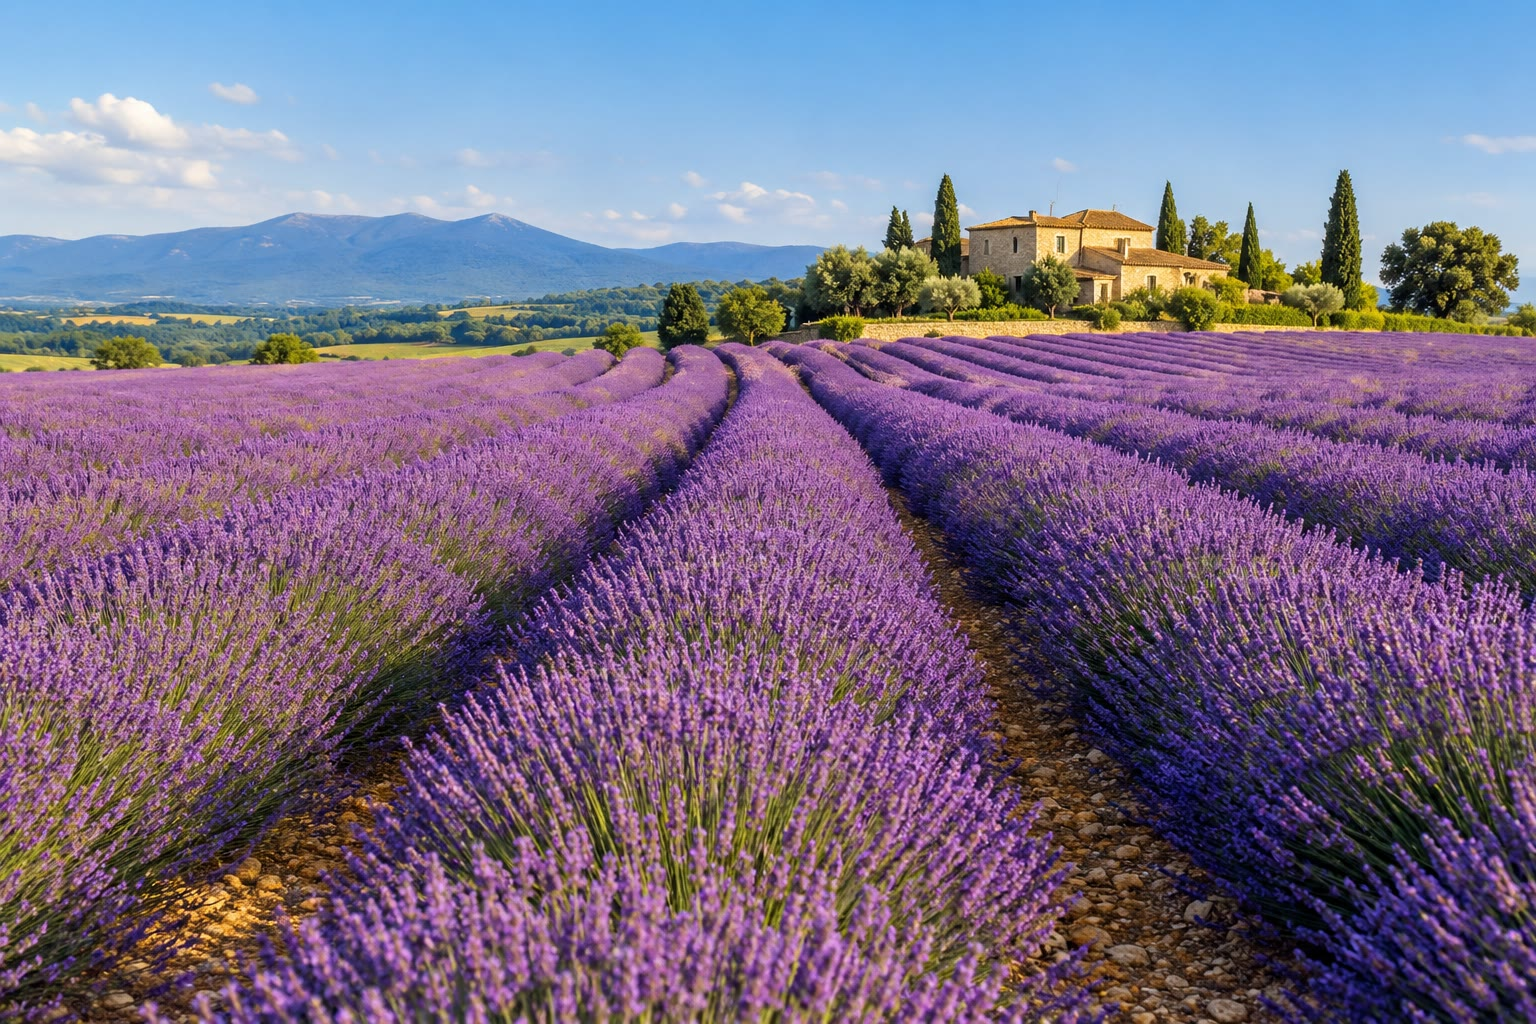
\includegraphics[width=0.55\linewidth]{images/book1/ai/g10-lavender-field.jpg}

{\small A lavender field in flower: the \omterm{def:g5:raw-materials-and-recycling:raw-material}{raw material} of lavender
essential oil.}
\end{omfigure}

\section{Exercises}

\begin{exercise}[$\star$]\label{exo:g10:chemical-species:1}
Natural or \omterm{def:g10:chemical-species:natural}{synthetic species}? Vanillin from a vanilla pod; aspirin;
caffeine from coffee beans; vanillin made in a factory.
\end{exercise}

\begin{exercise}[$\star$]\label{exo:g10:chemical-species:2}
Why do synthetic vanillin and natural vanillin have the same melting
point?
\end{exercise}

\begin{exercise}[$\star$]\label{exo:g10:chemical-species:3}
On a TLC plate, the \omterm{def:g6:solutions-and-solubility:solute}{solvent} front is \qty{6.0}{cm} above the starting line
and a spot is \qty{2.4}{cm} above it. Compute its $R_f$.
\end{exercise}

\begin{exercise}[$\star$]\label{exo:g10:chemical-species:4}
Give the role of the condenser in a \omterm{def:g10:chemical-species:distillation}{distillation}, and say why the cold
water enters at its lower end.
\end{exercise}

\begin{exercise}[$\star$]\label{exo:g10:chemical-species:5}
Name the three conditions an \omterm{def:g10:chemical-species:extraction}{extraction} \omterm{def:g6:solutions-and-solubility:solute}{solvent} must meet.
\end{exercise}

\begin{exercise}[$\star\star$]\label{exo:g10:chemical-species:6}
Using the table of \omterm{def:g6:solutions-and-solubility:solute}{solvents}, explain why ethanol cannot be used to
extract linalool from the distillate, while cyclohexane can.
\end{exercise}

\begin{exercise}[$\star\star$]\label{exo:g10:chemical-species:7}
In a separating funnel, dichloromethane is shaken with water. Which layer
is on top? Justify with the table.
\end{exercise}

\begin{exercise}[$\star\star$]\label{exo:g10:chemical-species:8}
A white powder sold as aspirin starts to melt at \qty{126}{\celsius} and
is fully melted at \qty{132}{\celsius}. What can you conclude?
\end{exercise}

\begin{exercise}[$\star\star$]\label{exo:g10:chemical-species:9}
Look at the TLC figure of this chapter. What does the lavender oil
contain? Which species climbed higher?
\end{exercise}

\begin{exercise}[$\star\star$]\label{exo:g10:chemical-species:10}
Put in order the steps of obtaining lavender oil in the laboratory:
separating the layers; \omterm{def:g10:chemical-species:distillation}{hydrodistillation}; adding cyclohexane to the
distillate and shaking; \omterm{def:g3:separating-mixtures:evaporate}{evaporating} the cyclohexane.
\end{exercise}

\begin{exercise}[$\star\star$]\label{exo:g10:chemical-species:11}
Why is the starting line of a TLC plate drawn in pencil and placed above
the \omterm{def:g10:chemical-species:tlc}{eluent}?
\end{exercise}

\begin{exercise}[$\star\star\star$]\label{exo:g10:chemical-species:12}
After \omterm{def:g10:chemical-species:extraction}{extraction}, the cyclohexane is removed by gentle heating, leaving
the oil. Using the boiling points of cyclohexane and of linalool, explain
why this works.
\end{exercise}

\begin{exercise}[$\star\star\star$]\label{exo:g10:chemical-species:13}
A synthetic sample of a flavour gives one spot on a TLC plate, at the
height of the \omterm{def:g10:chemical-species:natural}{natural species}, and melts sharply at the right
temperature. What two conclusions can you draw?
\end{exercise}

\begin{exercise}[$\star\star\star$]\label{exo:g10:chemical-species:14}
In the same TLC, spot A has $R_f = 0.40$ and the front is \qty{5.5}{cm}
above the line. At what height is spot A? Another species has
$R_f = 0.75$: how far above spot A is it?
\end{exercise}

\begin{exercise}[$\star\star\star$]\label{exo:g10:chemical-species:15}
\qty{1.6}{g} of linalool can \omterm{def:g2:mixing-and-dissolving:dissolve}{dissolve} in \qty{1}{L} of water. A distillate
of \qty{200}{mL} of water holds \qty{0.20}{g} of dissolved linalool. Is it
saturated? How much more could it \omterm{def:g2:mixing-and-dissolving:dissolve}{dissolve}? Why is it worth extracting
this water with cyclohexane rather than throwing it away?
\end{exercise}

\clearpage % keeps the heading with its problem box (it was stranded at a page foot)
\section{Problem: The Scent of Lavender}

\begin{problem}[{Weekend problem --- from a basket of lavender flowers to a
few drops of essential oil, checked by chromatography}]
\label{pb:g10:chemical-species:1}
% ledger: rho:cyclohexane, bp:cyclohexane, rho:CH2Cl2, bp:linalool, ghs:cyclohexane
In a school laboratory, \qty{100}{g} of fresh lavender flowers are
hydrodistilled with water. The distillate, cloudy, is shaken with
\qty{20}{mL} of cyclohexane in a separating funnel; the cyclohexane layer
is kept, dried, and the cyclohexane is evaporated by gentle heating. What
remains is lavender essential oil. Use the table of \omterm{def:g6:solutions-and-solubility:solute}{solvents} of this
chapter.

\medskip
\noindent\textbf{Part I --- The \omterm{def:g10:chemical-species:distillation}{hydrodistillation}.}
\begin{enumerate}
  \item What is the role of the boiling water in a \omterm{def:g10:chemical-species:distillation}{hydrodistillation}?
  \item What is the role of the condenser? Where does the cold water enter
        it?
  \item The distillate shows a thin oily layer floating on water. Is the
        oil \omterm{def:g6:solutions-and-solubility:miscible}{miscible} with water? Is it more or less dense than water?
  \item Why is the distillate not simply poured off to recover the oil?
\end{enumerate}

\medskip
\noindent\textbf{Part II --- The \omterm{def:g10:chemical-species:extraction}{extraction}.}
\begin{enumerate}[resume]
  \item Why is cyclohexane a suitable \omterm{def:g6:solutions-and-solubility:solute}{solvent} for this \omterm{def:g10:chemical-species:extraction}{extraction}?
  \item Could ethanol be used instead? Explain.
  \item After shaking and \omterm{def:g3:separating-mixtures:decant}{settling}, is the cyclohexane layer on top or at
        the bottom? What would it be with dichloromethane?
  \item Give two precautions required by the pictograms of cyclohexane.
  \item Why can the cyclohexane be evaporated without losing the
        linalool?
\end{enumerate}

\medskip
\noindent\textbf{Part III --- The chromatography.}
The oil, pure linalool (L) and pure linalyl ethanoate (A) are spotted on
a TLC plate. After development the front is \qty{6.0}{cm} above the
starting line. The oil gives two spots, at \qty{2.4}{cm} and
\qty{4.5}{cm}; spot L is at \qty{2.4}{cm}, spot A at \qty{4.5}{cm}.
\begin{enumerate}[resume]
  \item Compute the $R_f$ of linalool and of linalyl ethanoate.
  \item What does the oil contain, as far as this plate shows?
  \item Is lavender oil a \omterm{def:g6:pure-substances-and-mixtures:pure-substance}{pure substance}?
  \item Why were the references spotted on the same plate as the oil?
  \item A synthetic linalool is spotted on another plate run in the same
        conditions: its spot has $R_f = 0.40$. What can be concluded?
\end{enumerate}

\medskip
\noindent\textbf{Part IV --- How much oil?}
The oil obtained fills \qty{1.0}{mL}; \qty{1}{mL} of this oil weighs
\qty{0.90}{g}.
\begin{enumerate}[resume]
  \item What mass of oil was obtained?
  \item What percentage of the mass of the flowers is that?
  \item What mass of flowers would be needed for \qty{100}{g} of oil?
  \item The oil is said to be ``natural''. In what sense is this true? Is
        its linalool different from synthetic linalool?
  \item State the mass of essential oil obtained from \qty{100}{g} of
        flowers.
\end{enumerate}
\end{problem}
